\documentclass{csse4400}

% \teachermodetrue

\usepackage{float}
\usepackage{alltt}

\usepackage{languages}

\title{Databases in Applications}
\author{Brae Webb \& Evan Hughes}

\date{\week[practical]{2}}
\begin{document}

\maketitle

\begin{figure}[h]
  \href{https://www.oreilly.com/library/view/designing-data-intensive-applications/9781491903063/ch02.html}{
    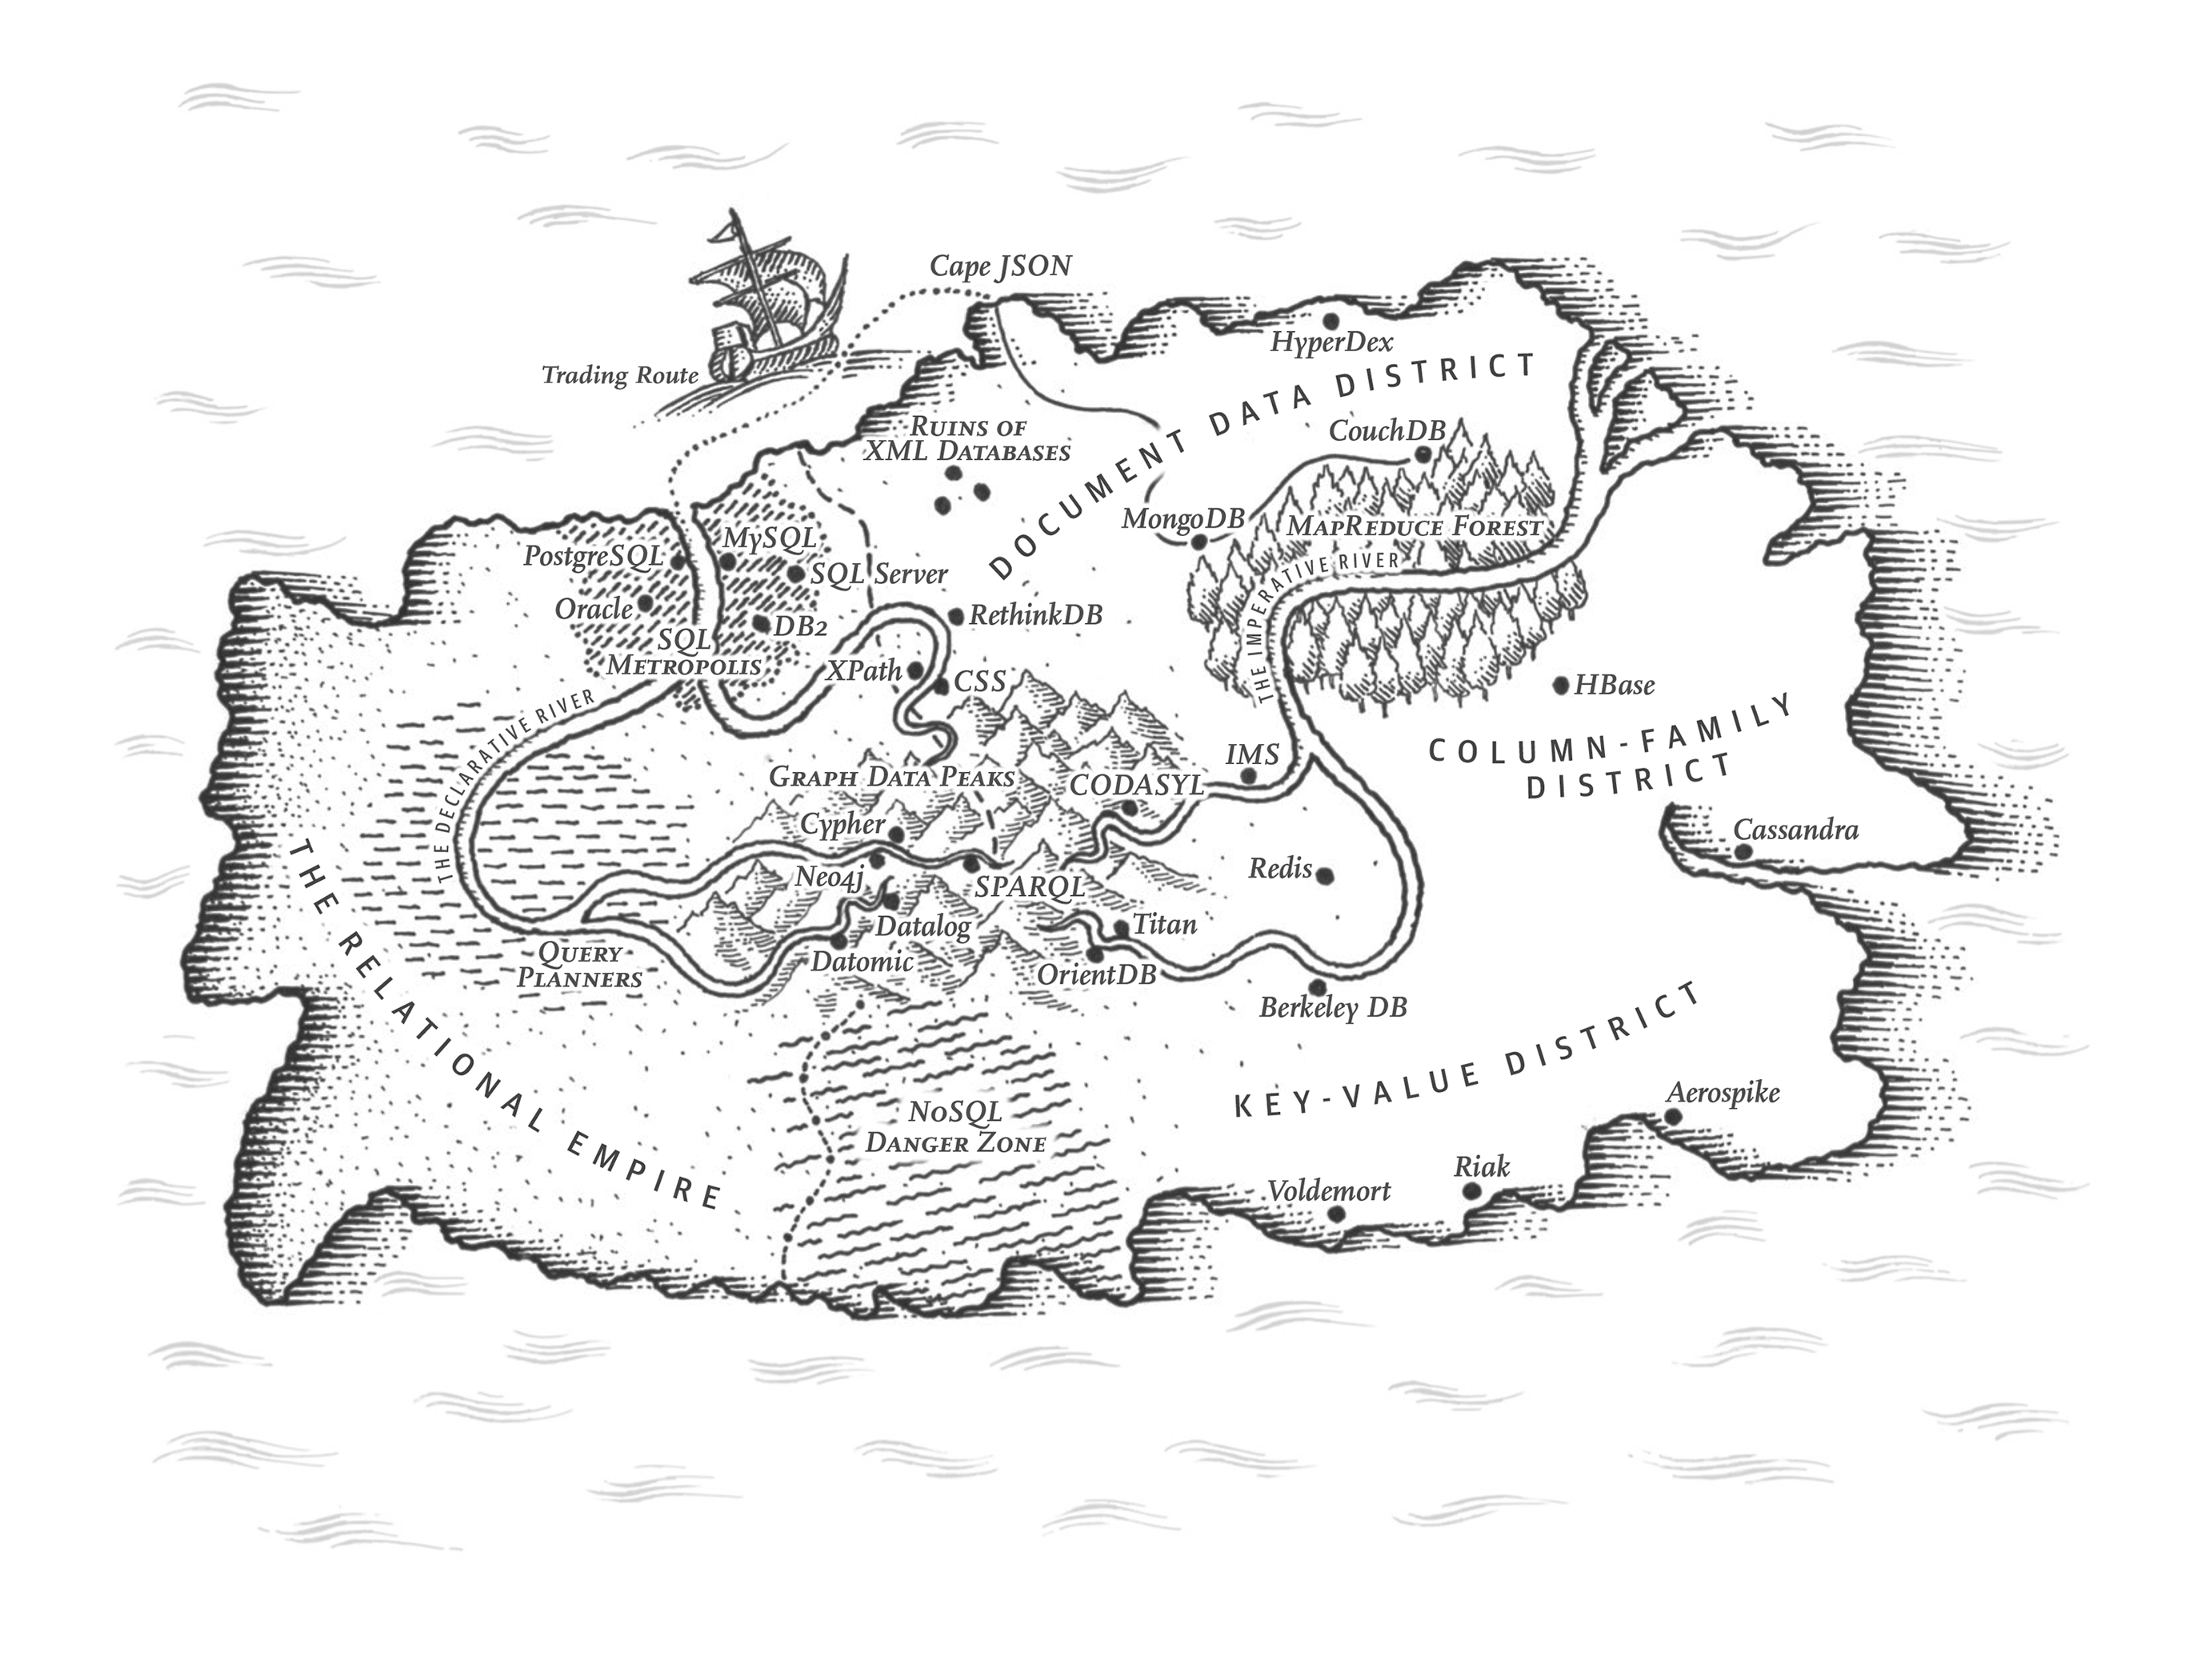
\includegraphics[width=\textwidth]{images/databases}
  }
\caption{A map of data storage techniques from Designing Data-Intensive Applications \cite{data-intensive}.}
\end{figure}

\aside{
  Github Classroom links for this practical can be found on Edstem \url{https://edstem.org/au/courses/15375/discussion/1753712}
}

\section{This Week}
This week our goal is to:
\begin{itemize}
  \item explore the various techniques developers use to store data; and
  %\item investigate the storage options implementing these techniques on the AWS platform;
  \item upgrade our todo application to use a local sqlite relational database.
\end{itemize}

\clearpage

\section{Databases and Data Models}
Unfortunately, to build interesting software we often need to store and use data.
The storage of data introduces a number of challenges when designing, creating, and maintaining our software.
However, not all data storage techniques are created equal;
the choice of data storage model can have a profound impact on our software's complexity and maintainability.
In this practical, we want to take a superficial exploration of our island of data storage models.
For a more in-depth treatment of data storage models that is outside the scope of this course,
see Chapter 2 of the \textit{Designing Data-Intensive Applications} book \cite{data-intensive}.


\teacher{
  Discuss the following different storage technologies and mention some use cases of when you would choose each one.
  Discuss some popular implementations of each.\\

  Aim for no more than 30 minutes of discussion.
}

\subsection{Relational Storage}

Relational databases are what you have been exposed to the most in your University career --- think MySQL, Postgres, Oracle DB, etc.
This type of database is good at modelling the real world which is often a highly connected environment.
% The data model that is suggested for this type of storage is a normalised approach where data duplication should be reduced.

Some popular offerings are below:

\begin{itemize}
  \item MySQL/MariaDB [ Amazon RDS / Amazon Aurora ].
  \item Postgres [ Amazon RDS / Amazon Aurora ].
  \item SQLite.
\end{itemize}

The AWS offerings of these services come in two different types, we have the traditional approach of
server capacity ( x cores, y ram ) and we have a server-less approach.
The server-less approach is a more dynamic
database that can scale to large amounts of load when needed though at a cost per request.

  \subsubsection{ORM}
  Object Relational Mapping (ORM) is a fairly common tool for programmers to use to make developing with databases smoother.
  One fairly prevalent example of this is SQLAlchemy which is a very widely used 
  database abstraction for python.
  SQLAlchemy allows us to move to a higher level of abstraction than SQL queries and perform database actions using standard python code.

  The benefits of ORMs are the ability to model database objects in our existing programming language instead of having large blocks of SQL text within our source code.
  The disadvantages come in when we need to do specific SQL work or where the abstractions cost is greater than the benefits.

\subsection{Wide-Column Storage}

\teacher{
  Examples of big apps that depend on this technology is Netflix \url{https://netflixtechblog.com/netflixs-viewing-data-how-we-know-where-you-are-in-house-of-cards-608dd61077da}.
}

Wide-Column databases are a form of NoSQL or non-relational data stores.
In these data stores the data model design 
is focused more on having efficient queries at the cost of data duplication.
A warning to the reader that these models
are not flexible after creation, it is much easier to answer a new use case in a relational model.

  \begin{itemize}
    \item Apache Cassandra [ Amazon Keyspaces for Cassandra ].
    \item Apache HBase.
  \end{itemize}

\subsection{Key-Value Storage}

Key-Value stores are very popular for cache or remote config use cases, some of the most notable are Redis and Memcached.
These stores allow efficient lookup of values via keys and are usually stored in-memory.

\begin{itemize}
  \item Redis [ Amazon ElastiCache for Redis ].
  \item Memcached [ Amazon ElastiCache for Memcached].
  \item Amazon DynamoDB.
  \item Amazon MemoryDB for Redis.
\end{itemize}

\subsection{Time Series Storage}

\teacher{
  Something to mention here is that relations are usually not utilised between tables in time series databases.
}

Time series databases are highly focused storage which is tailored to retrieving results by timestamp ranges.
Many implementations also take advantage of the data model to allow efficient rollover of data and partitioning.
One of the most popular time series databases is Prometheus which is used to store monitoring metrics.

\begin{itemize}
  \item Amazon Timestream.
  \item TimescaleDB ( Postgres + Addon ).
  \item Prometheus.
  \item InfluxDB.
  \item PostgreSQL
\end{itemize}

\subsection{Document Storage}

Document databases are a subset of NoSQL databases with a focus on a flexible data model.
MongoDB for instance allows the user to store JSON documents and perform queries on those documents.
One advantage of document databases is that they match a programmers existing mental model of storing data in formats such as JSON.

\begin{itemize}
  \item MongoDB.
  \item Apache CouchDB.
  \item Amazon DocumentDB.
  \item Amazon DynamoDB.
\end{itemize}

\subsection{Graph Storage}

\teacher{
  If you haven't experienced graph databases, a good usecase is ``recommendation systems'',
  which use the connected nature of items to figure out what to suggest to a person.
  Another example is the \url{https://neo4j.com/blog/analyzing-panama-papers-neo4j/}
  Panama Papers.
}

Graph Databases are relational storage with a few enhancements to allow fast neighbour look-ups.
These databases also allow the implementation of graph algorithms to query data.

\begin{itemize}
  \item Amazon Neptune.
  \item Neo4J.
  \item Janus Graph.
\end{itemize}

\begin{figure}[h]
  \href{https://neo4j.com/developer/example-project/}{
    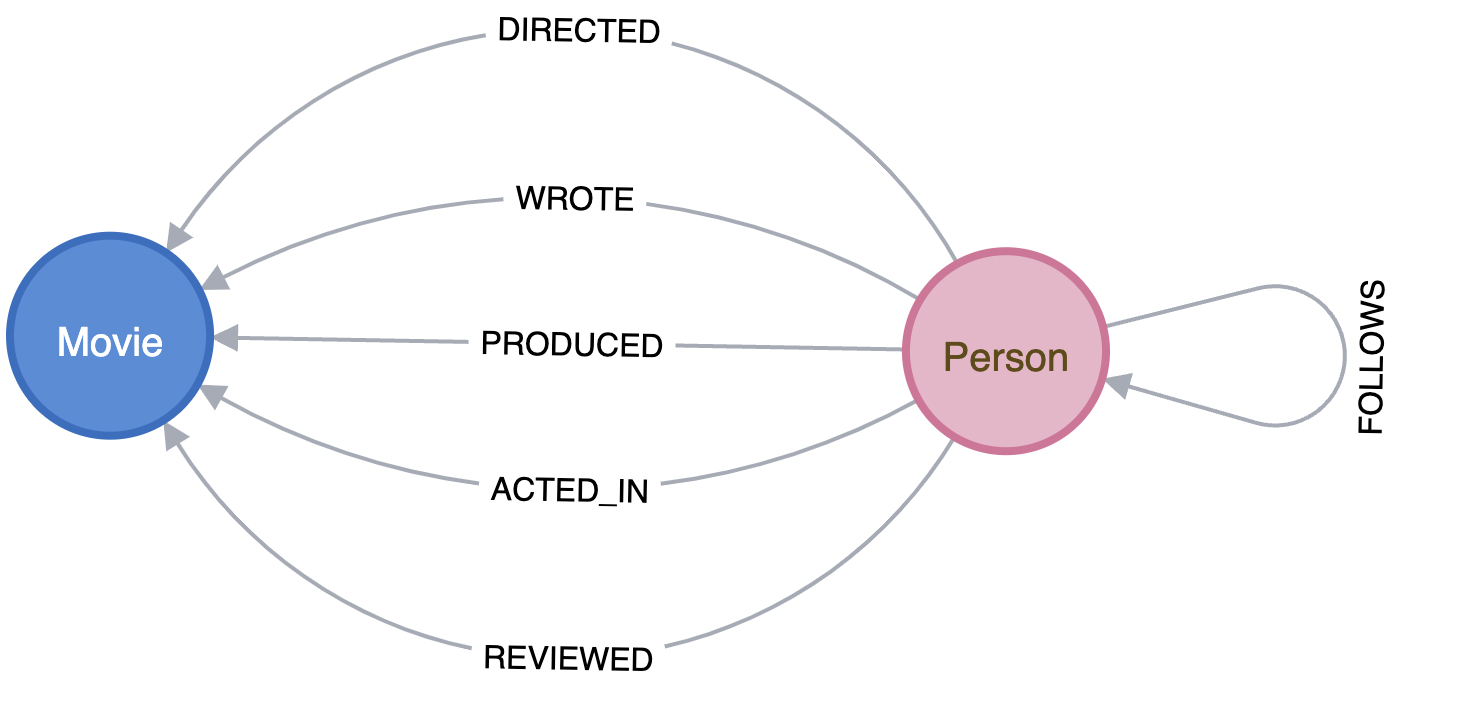
\includegraphics[width=\textwidth]{images/graph}
  }
  \caption{Graph Database Example from the Neo4J documentation.}
\end{figure}

\section{Enhancing the Todo App with Storage}

Last week we created a simple web server that can listen on a port and respond to HTTP requests.
The endpoints that we created are all stubs the return a hardcoded JSON response.
This week we will add a database to our application to support persistent storage.

\teacher{
  Pause here and let the students move around a bit while getting their repos setup.
}

\subsection{Creating a Practical Repository}
Navigate to the GitHub Classroom link for this practical provided on the EdStem discussion board.
As with last week, this will create a new repository for you in the course organisation.
You can now clone this repository to your local machine or work directly in the browser with GitHub codespaces.
This repository will be populated with our solution to last weeks practical exercise.
You may modify this solution or replace it with your own.

% \info{
%   If using Github CodeSpaces the environment will be pre-installed with the libraries you used last week.
%   You will still need to follow on with the instructions below to install the database libraries.
% }

\subsection{Installing the Database Dependencies}

We will be using a Python library called SQLAlchemy to interact with our database.
This library abstracts the SQL queries away and allows us to interact with the database using Python objects.
We will be using SQLAlchemy using a package called Flask-SQLAlchemy, a wrapper around SQLAlchemy,
that is designed to work with Flask our WebServer library.

\bash{poetry add flask-sqlalchemy}

\subsection{Creating the Database and Models}

We will be using a database called SQLite for this practical.
SQLite is a file-based database which is easy to setup and use.
As the database is isolated to a file, SQLite is a good choice for initial development.

Now that our dependencies are installed,
navigate to the cloned practical directory and create a new folder within the todo folder called \texttt{models}.
Inside this folder create a new file called \texttt{todo.py} and a new file called \texttt{\_\_init\_\_.py}.

Inside the \texttt{\_\_init\_\_.py} file we will add the following code:

\begin{code}[language=python,numbers=none]{}
  from flask_sqlalchemy import SQLAlchemy

  db = SQLAlchemy()
\end{code}

All this file does is setup a new SQLAlchemy object which we will use to interact with our database.
In the \texttt{models/todo.py} file we will add the following code:

\begin{code}[language=python,numbers=none]{}
import datetime
from . import db

class Todo(db.Model):
    __tablename__ = 'todos'

    # This is how we define a column, this is also the primary key
    id = db.Column(db.Integer, primary_key=True)
    # This is a manadatory column of 80 characters
    title = db.Column(db.String(80), nullable=False)
    # This is an optional column of 120 characters
    description = db.Column(db.String(120), nullable=True)
    # This column has a default value of False
    completed = db.Column(db.Boolean, nullable=False, default=False)
    deadline_at = db.Column(db.DateTime, nullable=True)
    # This column has a default value which is a function call
    created_at = db.Column(db.DateTime, nullable=False, default=datetime.datetime.utcnow)
    # This column has a default value which is a function call and also updates on update
    updated_at = db.Column(db.DateTime, nullable=False, default=datetime.datetime.utcnow, onupdate=datetime.datetime.utcnow)
    
    # This is a helper method to convert the model to a dictionary
    def to_dict(self):
        return {
            'id': self.id,
            'title': self.title,
            'description': self.description,
            'completed': self.completed,
            'deadline_at': self.deadline_at.isoformat() if self.deadline_at else None,
            'created_at': self.created_at.isoformat() if self.created_at else None,
            'updated_at': self.updated_at.isoformat() if self.updated_at else None,
        }

    def __repr__(self):
        return f'<Todo {self.id} {self.title}>'
\end{code}

The above code is doing a lot of the heavy lifting for us in our database table generation,
have a look at the comments above to see what each line is doing.


\subsection{Configuring the Database}

Now that we have defined our database schema using an ORM,
we need to configure our application to use the database.
Open the \texttt{todo/\_\_init\_\_.py} file and change the code to the following:

\begin{code}[language=python,numbers=none]{}
from flask import Flask
from flask_sqlalchemy import SQLAlchemy

def create_app():
    app = Flask(__name__)

    app.config['SQLALCHEMY_DATABASE_URI'] = "sqlite:///db.sqlite"

    # Load the models
    from todo.models import db
    from todo.models.todo import Todo
    db.init_app(app)

    # Create the database tables
    with app.app_context():
        db.create_all()
        db.session.commit()

    # Register the blueprints
    from todo.views.routes import api
    app.register_blueprint(api)

    return app
\end{code}

In the above we set a default location, defined as a URI, for our database.
As we using SQLite we can set the database to be a file on the file system.
In production systems, you would set this to a URI that defines the credentials and hostname of your database server.
In latter practicals, we will get experience using more complex URIs.

If we run our application now, we will see that the database file has been created for us.
\bash{poetry run flask --app todo run -p 6400 --debug}

\pagebreak

Your project structure should have a least the follow structure (there may be additional files):

\begin{code}[language=bash,numbers=none]{}
-- README.md
-- Pipfile
-- Pipfile.lock
-- endpoints.http
-- instance
  | -- db.sqlite
-- todo
  | -- __init__.py
  | -- views
      | -- routes.py
  | -- models
      | -- __init__.py
      | -- todo.py
\end{code}

\subsection{Inspecting the Database}

We can use the \texttt{sqlite3} command line tool to inspect the database.
Open a terminal and navigate to the root of your project.
Then run the following command:

\bash{sqlite3 instance/db.sqlite}

\info{
  Most platforms including MacOS, WSL2, and most Linux environments come with SQLite installed.
  If you get an error running the above command, you may have to install SQLite.
}

This will open the SQLite command line tool and connect to the database file.
We can then run the following command to see the tables in our database:

\begin{code}[language=sql,numbers=none]{}
  .tables
\end{code}

This will show us the tables in our database.
We can then run the following command to see the schema of our table:

\begin{code}[language=sql,numbers=none]{}
  .schema todos
\end{code}

This will show us the columns in our table.
We can then run the following command to see the data in our table:

\begin{code}[language=sql,numbers=none]{}
  SELECT * FROM todos;
\end{code}

This should initially show us no output, indicating that the table is currently empty.
We can then run the following command to exit the SQLite command line tool:

\begin{code}[language=sql,numbers=none]{}
  .exit
\end{code}

You should notice that our table is called todos and not todo because we specified todos with the \texttt{\_\_tablename\_\_} attribute.


\subsection{Using the Database}

Now that we have a database intergrated into our application,
we will modify our endpoints to take advantage of it. 

Open the \texttt{todo/views/routes.py} file and add the following imports to the top of the file:

\begin{code}[language=python,numbers=none]{}
from flask import Blueprint, jsonify, request
from todo.models import db
from todo.models.todo import Todo
from datetime import datetime
\end{code}

Open the \texttt{todo/views/routes.py} file and change the \texttt{get\_todos} endpoint to the following:

\begin{code}[language=python,numbers=none]{}
@api.route('/todos', methods=['GET'])
def get_todos():
    todos = Todo.query.all()
    result = []
    for todo in todos:
        result.append(todo.to_dict())
    return jsonify(result)
\end{code}

This will query the database for all the todos and return them as JSON.
We can then change the \texttt{get\_todo} endpoint to the following:

\begin{code}[language=python,numbers=none]{}
@api.route('/todos/<int:todo_id>', methods=['GET'])
def get_todo(todo_id):
    todo = Todo.query.get(todo_id)
    if todo is None:
        return jsonify({'error': 'Todo not found'}), 404
    return jsonify(todo.to_dict())
\end{code}

Now we have modified these endpoints to use the database --- let's test that our application is still functioning correctly.
Restart your webserver and navigate to the \texttt{/api/v1/todos} endpoint.
You should see the following JSON response:

\begin{code}[language=json,numbers=none]{}
  []
\end{code}

Of course our API does not have any todo items in it yet.
We will now add the ability to insert todo items to our database.
Open the \texttt{todo/views/routes.py} file and change the \texttt{create\_todo} endpoint to the following:

\begin{code}[language=python,numbers=none]{}
@api.route('/todos', methods=['POST'])
def create_todo():
    todo = Todo(
        title=request.json.get('title'),
        description=request.json.get('description'),
        completed=request.json.get('completed', False),
    )
    if 'deadline_at' in request.json:
        todo.deadline_at = datetime.fromisoformat(request.json.get('deadline_at'))

    # Adds a new record to the database or will update an existing record
    db.session.add(todo)
    # Commits the changes to the database, this must be called for the changes to be saved
    db.session.commit()
    return jsonify(todo.to_dict()), 201
\end{code}

This endpoint now allows us create a todo item in the database.
Test this endpoint by going to endpoints.http (or your API query tool of choice) and running the POST request.
You should see the following response (with different created\_at and updated\_at values):

\begin{code}[language=json,numbers=none]{}
  {
    "id": 1,
    "title": "Test Todo",
    "description": "This is a test todo",
    "completed": false,
    "deadline_at": null,
    "created_at": "2023-02-27T12:00:00.000000Z",
    "updated_at": "2023-02-27T12:00:00.000000Z"
  }
\end{code}

Now if we go to our \texttt{/api/v1/todos} endpoint we should see the todo item we just created:

\begin{code}[language=json,numbers=none]{}
  [
    {
      "id": 1,
      "title": "Test Todo",
      "description": "This is a test todo",
      "completed": false,
      "deadline_at": null,
      "created_at": "2023-02-27T12:00:00.000000Z",
      "updated_at": "2023-02-27T12:00:00.000000Z"
    }
  ]
\end{code}

Now let's add the remaining endpoints.
Change the \texttt{update\_todo} endpoint to the following:

\begin{code}[language=python,numbers=none]{}
@api.route('/todos/<int:todo_id>', methods=['PUT'])
def update_todo(todo_id):
    todo = Todo.query.get(todo_id)
    if todo is None:
        return jsonify({'error': 'Todo not found'}), 404

    todo.title = request.json.get('title', todo.title)
    todo.description = request.json.get('description', todo.description)
    todo.completed = request.json.get('completed', todo.completed)
    todo.deadline_at = request.json.get('deadline_at', todo.deadline_at)
    db.session.commit()

    return jsonify(todo.to_dict())
\end{code}

This endpoint will update a todo item in the database.
Let's test this endpoint by going to our endpoints.http and running the PUT request.
You should see the following response:

\begin{code}[language=json,numbers=none]{}
  {
    "id": 1,
    "title": "Updated Test Todo",
    "description": "This is an updated test todo",
    "completed": false,
    "deadline_at": null,
    "created_at": "2023-02-27T12:00:00.000000Z",
    "updated_at": "2023-02-27T12:00:00.000000Z"
  }

\end{code}

To implement delete functionalitty, we will use the HTTP DELETE method and the delete .method of the database session.
Open the \texttt{todo/views/routes.py} file and change the \texttt{delete\_todo} endpoint to the following:

\begin{code}[language=python,numbers=none]{}
@api.route('/todos/<int:todo_id>', methods=['DELETE'])
def delete_todo(todo_id):
    todo = Todo.query.get(todo_id)
    if todo is None:
        return jsonify({}), 200

    db.session.delete(todo)
    db.session.commit()
    return jsonify(todo.to_dict()), 200
\end{code}

We now have a set of endpoints that can perform the CRUD operations of our API but some functionality is missing.
We are gonna add that functionality after setting up some tests to help us do \textbf{Test Driven Development}.

\section{Testing the API}

\subsection{Setting up the testing environment}

In the project, you will have a \texttt{tests} folder.
This contains \texttt{test\_todo.py} which has a range of provided tests for the todo endpoints.
However, we need to setup a few components to make it work.

Inside the \texttt{tests} folder create a \texttt{base.py} file. Inside the \texttt{base.py} file add the following code:

\begin{code}[language=python,numbers=none]{}
  from todo import create_app
  import unittest
  
  
  class TodoTest(unittest.TestCase):
      def setUp(self):
          self.app = create_app(config_overrides={
              'SQLALCHEMY_DATABASE_URI': 'sqlite:///:memory:',
              'TESTING': True
          })
  
          self.client = self.app.test_client()
  
      def assertDictSubset(self, expected_subset: dict, whole: dict):
          for key, value in expected_subset.items():
              self.assertEqual(whole[key], value)
\end{code}


This base class is what we will use to help setup our tests and provide an assertion helper method.
The \texttt{setUp} method is called before each test and is used to initialise the in-memory database.
The \texttt{assertDictSubset} method is a helper method that we will use to compare the todo items we get from the API with the todo items we expect to get from the API.

As you can see we use a slight modification to the \texttt{create\_app} function.
We are passing in a dictionary of config overrides.
This allows us to override the config values for the testing environment.

\subsection{Prepping the config for testing}

Open the \texttt{todo/\_\_init\_\_.py} file and adjust the \texttt{create\_app} function to the following:

\begin{code}[language=python,numbers=none]{}
  def create_app(config_overrides=None):
      app = Flask(__name__)
  
      app.config['SQLALCHEMY_DATABASE_URI'] = "sqlite:///db.sqlite"
      if config_overrides:
          app.config.update(config_overrides)
          
      # Load the models
      from todo.models import db
      from todo.models.todo import Todo
      db.init_app(app)
  
      # Create the database tables
      with app.app_context():
          db.create_all()
          db.session.commit()
  
      # Register the blueprints
      from .views.routes import api
      app.register_blueprint(api)
  
      return app
\end{code}

\subsection{Writing our first tests}

Now we will write our first tests.
Open the \texttt{tests} folder and create a \texttt{test\_health.py} file.
Add the following code:

\begin{code}[language=python,numbers=none]{}
  from tests.base import TodoTest
  
  
  class TestHealth(TodoTest):
      def test_health(self):
          response = self.client.get('/api/v1/health')
          self.assertEqual(response.status_code, 200)
          self.assertEqual(response.json, {'status': 'ok'})

\end{code}

This test will make a GET request to the \texttt{/api/v1/health} endpoint and check 
\begin{itemize}
  \item that the response is a 200 status code; and
  \item that the response is a JSON object with the key \texttt{status} and the value \texttt{ok}.
\end{itemize}

To run this test stop your server, if it is running, and run the following command:

\bash{poetry run python3 -m unittest tests/test_health.py}

You should see the following output:

\begin{code}[language=bash,numbers=none]{}
  >> poetry run python3 -m unittest tests/test_health.py
  ....
  ----------------------------------------------------------------------
  Ran 1 tests in 0.011s

  OK
\end{code}

\subsection{Test Driven Development}

Now you've created a test for the health endpoint and run it.
To run the suite of provided tests,
use the following command:

\bash{poetry run python3 -m unittest discover -s tests}

If you've used only the code we've provided,
you should see some of the tests fail.

The tests are based on the specification from week one,
we would like you to change your API to make the tests pass.

\hint{
To check if the request is a JSON request you can use the \texttt{request.is\_json} method.
}

If you get stuck feel free to ask your peers / staff for help.

\section{Finishing Up}

We now have a working API which we can use to create, read, update, and delete todo items.
We can also use the API to:
\begin{itemize}
  \item mark todo items as completed;
  \item filter todo items by whether they are completed or not (a query parameter of completed in the list get query); and
  \item filter todo items by whether they are within the next N days. In the tests this is exposed by a query parameter \texttt{window}.
\end{itemize}

Next week we will dockerise our API and use docker-compose to run our API and a database within containers.

\bibliographystyle{ieeetr}
\bibliography{books,ours}

\end{document}
